\documentclass{article}
\usepackage{url}
\usepackage{longtable}
\usepackage{graphicx}
\usepackage{multirow}
\title{Word Sense Disambiguation\\
\small{Leveraging the NLTK Toolkit and External Tools}}
\author{
Alec Story
Ansu Abraham
Craig Frey\\
Dustin Tiedemann
Michael Zhu
Thomas Levine
Whitney Foster\\
}

\newcommand{\naive}{na\"ive}
\newcommand{\Naive}{Na\"ive}

\begin{document}
\maketitle

\section{Overview}

We  chose to implement our system in Python, and chose to use the machine
learning algorithms in NLTK which is also Python-based.  We also used NLTK for
its part of speech tagger, dependency parser, and to import the Senseval data.
We coded the rest of the assignment on our own.

We wrote our main control program, classify.py, so that it can choose either
\Naive{} Bayes or Decision Trees classifier and any 
combination of  features. On top of this we wrote bash scripts that automated
looping through every combination of classifiers and features, along with
porting the results directly into the scorer.  Classify.py includes a help
switch -h, that explains the switches that control the different classifiers
and features along with any additional parameters that a certain feature might
support (for example, collocation has a window size parameter which defaults to
0) Performance was excellent for most of the features, allowing us to typically
run all of the words in the test set through every combination a classifier and
feature set in under an hour. (The number of runs can get quite high when you
factor in several parameters per feature, not just on/off)

A baseline was run by choosing the most frequent sense for each word.

\subsection{Data details}

The NLTK has a corpus reader that imports Senseval-2 files. The Senseval-3
file format is slightly  different which necessitated a few changes. We
separated the training  and test files by word into .pos files to match  what
the existing parser looked for. In the interest of time we modified  the
training and test files to contain a single tagged word per chunk (but still
allowing for multiple senses) again to match the Senseval-2  format.

\subsection{Selecting optimal feature combination}
\newcommand\ward{backward} %or maybe backwards

We used a \ward stepwise approach to identifying optimal feature combinations.
We first ran the system with all features on, producing a total of $256=2^8$
combinations.  We then used backwards stepwise regression to identify feature
combinations with a small number of features but with high performance

\section{System}

We made heavy use of python's NLTK
package\footnote{\url{http://www.nltk.org/}}, using its classifiers as our
machine learning engines, and several of its other packages for analysis.

\subsection{Classifiers}

The NLTK was used to implement two machine learning algorithms, \naive{} Bayes and
decision trees.  

\subsubsection{\Naive{} Bayes}

The NLTK implements a \naive{} Bayes classifier which chooses the best sense given a
dictionary of features and assigns confidence probabilities to the chosen
sense. \Naive{} Bayes does assume an independence of features. The probability of
each feature contributes to the overall choice.

\subsubsection{Decision Tree}

The NLTK also implements a decision list classifier in which a sequence of
tests is applied to each target-word feature vector. Each test indicates a
particular sense of the word: if the test succeeds, the sense of the test is
returned otherwise the next test in the sequence is performed.

\Naive{} Bayes supported probability estimation, while the decision tree did not.

\subsection{Confidence Cutoffs}

NLTK provides probability measures for each of its guesses when using the
maximum entropy and the \naive{} Bayes learning methods.  We harnessed these to
determine the cutoff for making a guess, or resorting to a ``U'' if we were not
confident in the tagging.  Occasional unknowns also occur because such unknowns
are present in the training data, and we made no effort to remove them, so the
learning algorithm views them as any other label.  Where we used confidence
cutoffs, we used .5 as our cutoff.

% Should we mention which cutoff we used?  Which did we use?

\subsection{Bootstrapping}

We used the same probability measure from the confidence cutoffs to fuel a
bootstrapping method.  Instead of directly taking the output of the classifier,
we instead looked at its performance on the test data, and wherever it was very
confident, we copied that test instance to the training data, and repeated this
cycle for a fixed number of cycles.  Once we had enriched the training data, we
ran the classifier a final time to perform classification.

Fortunately, the classifiers were very fast, and almost all of the time the
system spends is in reading input and building feature sets, which don't need
to be repeated, so bootstrapping is very cheap to include.  The probability measure that we used for the algorithm was 0.8

% Should we mention which probability measure we used?  Which did we use?  How
% many iterations?


\subsection{Base Word}

Because the target words were grouped by part of speech, we included the word
as it appears literally in context as a feature.  For example, ``activate''
versus ``activating,'' which both appear under activate.v.

\subsection{Dependency Parsing}

We included as one feature the MaltParser dependency parser, and used the
engmalt.linear.mco linear support vector machine
configuration\footnote{\url{http://maltparser.org/mco/english_parser/engmalt.html}}
for parsing (the other option was an SVM with a polynomial kernel, which the
Malt website said would run just as accurately, more slowly, but with less
memory, so we decided to go with the faster option).

From the parser we rendered several features:

\begin{description}

\item[The Dependency:] whatever the first of the list of dependencies given for
the target word is.  It is difficult to represent lists in the key and value
feature format, so we did not attempt to.  Instead, we use the rest of the
features as mitigating factors.  The empty string if there is no dependency.

\item[Presence of Absence of Dependency]

\item[Number of Dependencies]

\item[The Parent:] the word with the target word as (one of) its dependencies.

\end{description}

Dependency parsing is fairly slow, requiring about a second per instance to run
on a computer running an Atom D525 processor (which is fairly underpowered, but
modern).  To help alleviate this problem, we wrote a system that saves parses
for each context, and only calls the parser if it observes a new parse, so we
could reuse parsing information across runs of our program.  Because this file
is several hundred megabytes in size, it is not included in our
submitted code.

\subsection{Collocation}

Encodes the part-of-speech tag of words to the left and right of the target
word. The number of words extracted is determined by a variable window size
(context) which the function takes in as an input. Half the window size is
taken from left the word and half from the right of the word; thus window size
is the total number of words examined. For an odd window size, it rounds up
half the window size up for the part left of the word and rounds down for the
part right of the word.

We rendered a feature for each position covered, and set its value to be the
word at that position.

We also used NLTK's part of speech tagger to tag the context, and included those
as we did the literal words in the feature set.  This was trained on NLTK's
\verb+maximum entropy treebank pos tagger+ data, which is included with the NLTK
package.

\subsection{Co-occurrence}

Looks through the training data and compiles a list of most common words for
each item in the data. When the test data is run, the feature looks for the
created vector and uses that instead of trying to make a new one. Next the
extractor takes a window of words around the head word and generates the 0, 1
tuple of features for inclusion to the dictionary. This word list is used as the
keys of the feature vector when using the test data as a list of words that may
co-occur with each item in the data. The value associated with each key in the
feature vector starts out as 0 (for occurring 0 times in the window near a test
word) If a key in the feature vector does occur with a word in the test data,
the value associated with the key changes to 1 even if the key occurs more than
once.  This is necessary because the machine learning algorithm we used does not
attempt to analyze the keys beyond simple equality, so higher numbers than one
could have masked the possibly more important distinction between 0 and not-0.
In other words, keeping track of the instances of occurrence vs clustering them
into 2 groups reduces the sparsity of the data and allows for a higher chance of
accurate classifications based on the limited training data that we have. This
is an especially important consideration since the feature vectors that select
the most common words by looking through all the instances of unique lexical
items in the training data are unsupervised.

\section{Methods}
\newcommand\few{few}

We ran the system with several hundred different combinations of features over
all the words in the input set.

We identified optimal feature combinations through backward stepwise simple
linear regression and through the creation and visual analysis of charts. The
former has the advantage of discovering relationships and testing them more
quantitatively but has the disadvantage of making assumptions about normality,
linearity and equal variance.  The latter has the advantage of elucidating more
complex and higher-order relationships.

We ran a more detailed analysis on the top \few systems.  This analysis included
consideration of all three grain-levels of score and scores by word.

\section{Results}

\subsection{Stepwise regression}

We ran backward stepwise regression with the F-measure from the coarse-grained
scores regressed on predictors representing the feature combination.  The
saturated model contained the following predictors and all interactions

\begin{itemize}
\item Classifier (\naive{} Bayes or decision list)
\item Collocation window length (0--8)
\item Co-occurrence handling (on or off)
\item Base word handling (on or off)
\item Bootstrap iterations (0--4)
\item Dependency parsing (on or off)
\end{itemize}

The predictor combination yielding the lowest value of the Akaike information criterion
included the following parameters.

\begin{itemize}
\item Intercept
\item Classifier
\item Collocation window size
\item Co-occurrence
\item Base word handling
\item Classifier$\times$collocation window size interaction
\item Classifier$\times$co-occurrence interaction
\end{itemize}

This does not include bootstrap iterations, indicating that changes
in bootstrap iterations does not substantially change the F-measure.

%Discuss the coefficients in the regression table
%Call:
%lm(formula = f ~ classifier + collocation + cooccurrence + base_word +     dependency_parsing + classifier:collocation + classifier:cooccurrence +     collocation:cooccurrence + collocation:dependency_parsing +     cooccurrence:dependency_parsing + collocation:cooccurrence:dependency_parsing,     data = plot.step.import())

Coefficients:

\begin{tabular}{l r}
                                (Intercept) & 0.5557355 \\
                                classifiert & 0.0444331  \\
                                 collocation & 0.0030636  \\
                              cooccurrence1 & 0.0276413 \\
                                 base word1 & 0.0124008  \\
                         dependency parsing & -0.0019423 \\
                     classifiert:collocation & -0.0132109 \\
                  classifiert:cooccurrence1 & -0.0271825 \\
                   collocation:cooccurrence1 & -0.0007417 \\
              collocation:dependency parsing & -0.0003464 \\
           cooccurrence1:dependency parsing & -0.1611043 \\
collocation:cooccurrence1:dependency parsing & 0.0147078  \\
\end{tabular}

As the regression table above shows, it seems that substituting the
Decision Tree classifier for the Naive Bayes baseline provides the
most significant boost to our f measure. It can also be seen here that
increasing the collocation window will increase the f measure by about 0.003
for each additional word added to the window. Additionally, enabling
the cooccurrence feature extractor with the Naive Bayes classifier
will increase the f measure by a significant amount as well.

The rows that contain negative terms may indicate that the interacting
features provide similar functionality. That is, the enabled features
are interfering with each other so that their final influence on the f
measure may affect the f measure negatively. For instance, the row
showing ``classifiert:collocation'' indicates a run where the Decision
Tree classifier was used and the collocation feature was enabled has
resulted in a lower accuracy. This seems to be the general trend for
all of the interacting features. It may be interesting to note that
the interaction between collocation and cooccurrence1 as well as
collocation and dependency parsing produce the most innocuous
cumulative effect. Perhaps this may be why collocation and
cooccurrence are often advocated to be used together.

\subsection{Graphical methods}
We began by plotting the predictors that seemed most influential in the
stepwise regression.

\begin{figure}[H]
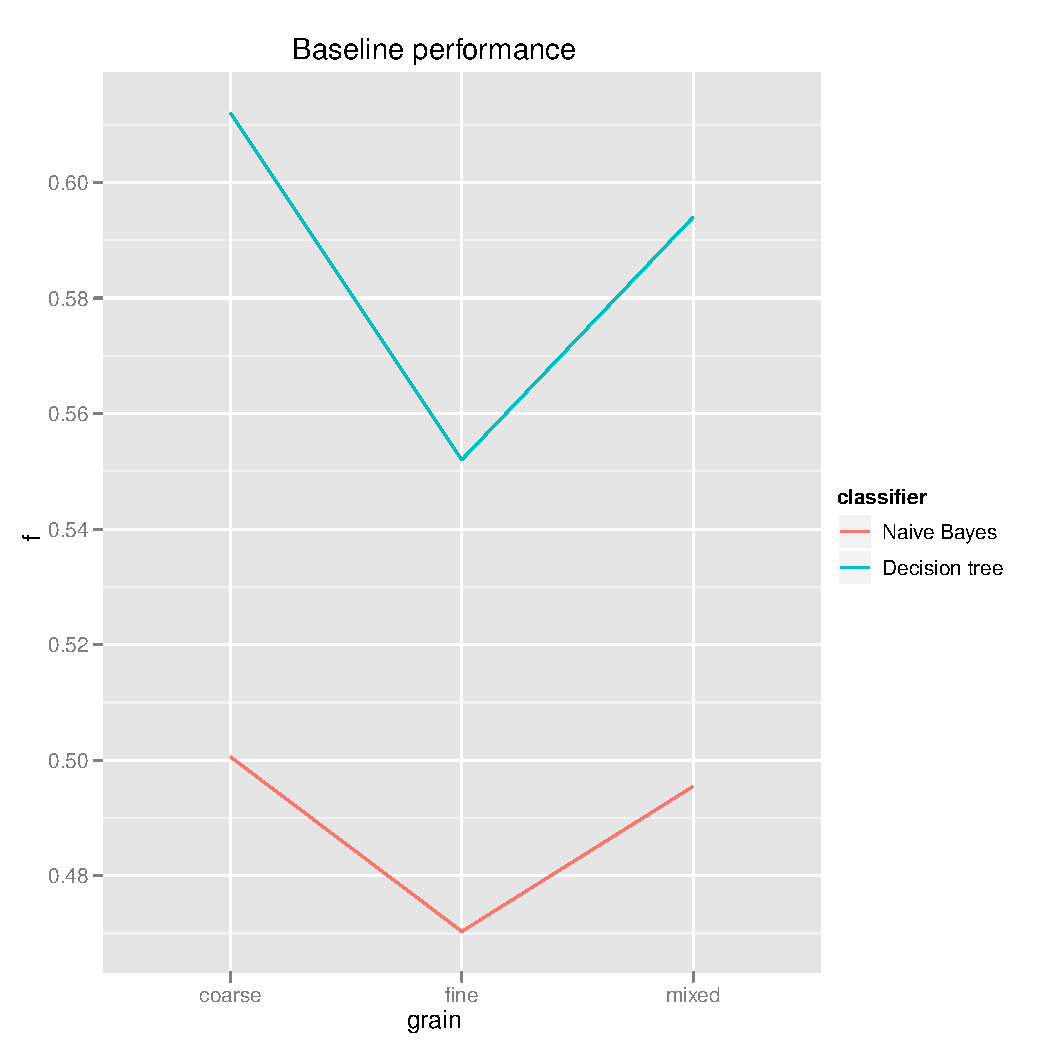
\includegraphics[width=\textwidth]{baseline}
\caption{\label{fig:base}Baseline scores for our two baseline systems}
\end{figure}

Figure \ref{fig:base} shows our results for running just the Decision
Tree classifier and the \naive{} Bayes classifier with no features
enabled. With no bootstrapping, the Decision Tree classifier has a
much higher f-measure. With bootstrapping, the Decision Tree
classifier decreases in f-measure while the \naive{} Bayes classifier
improves in f-measure.

<<<<<<< HEAD
%\begin{figure}
%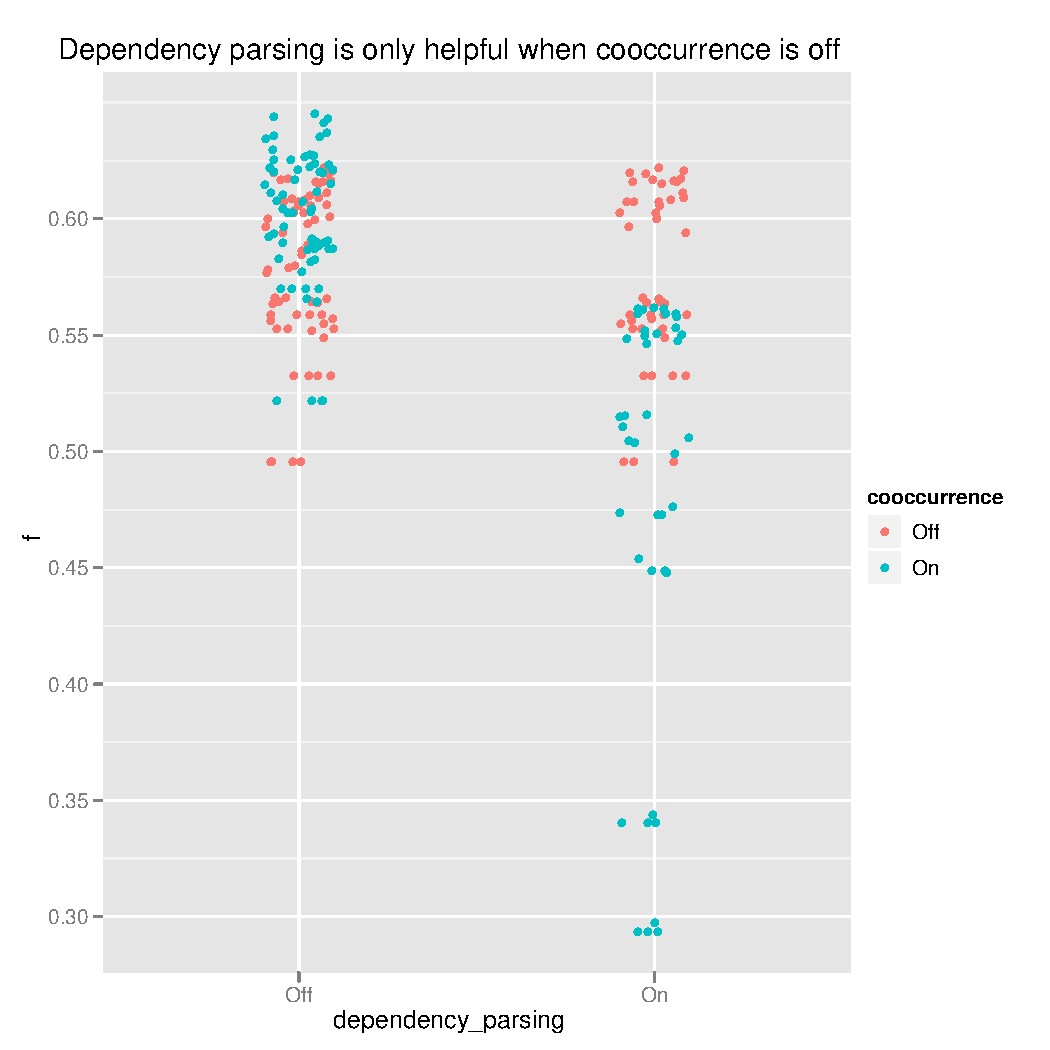
\includegraphics[width=\textwidth]{pg_0001}
%\caption{\label{fig1}}
%\end{figure}
=======
\begin{figure}[H]
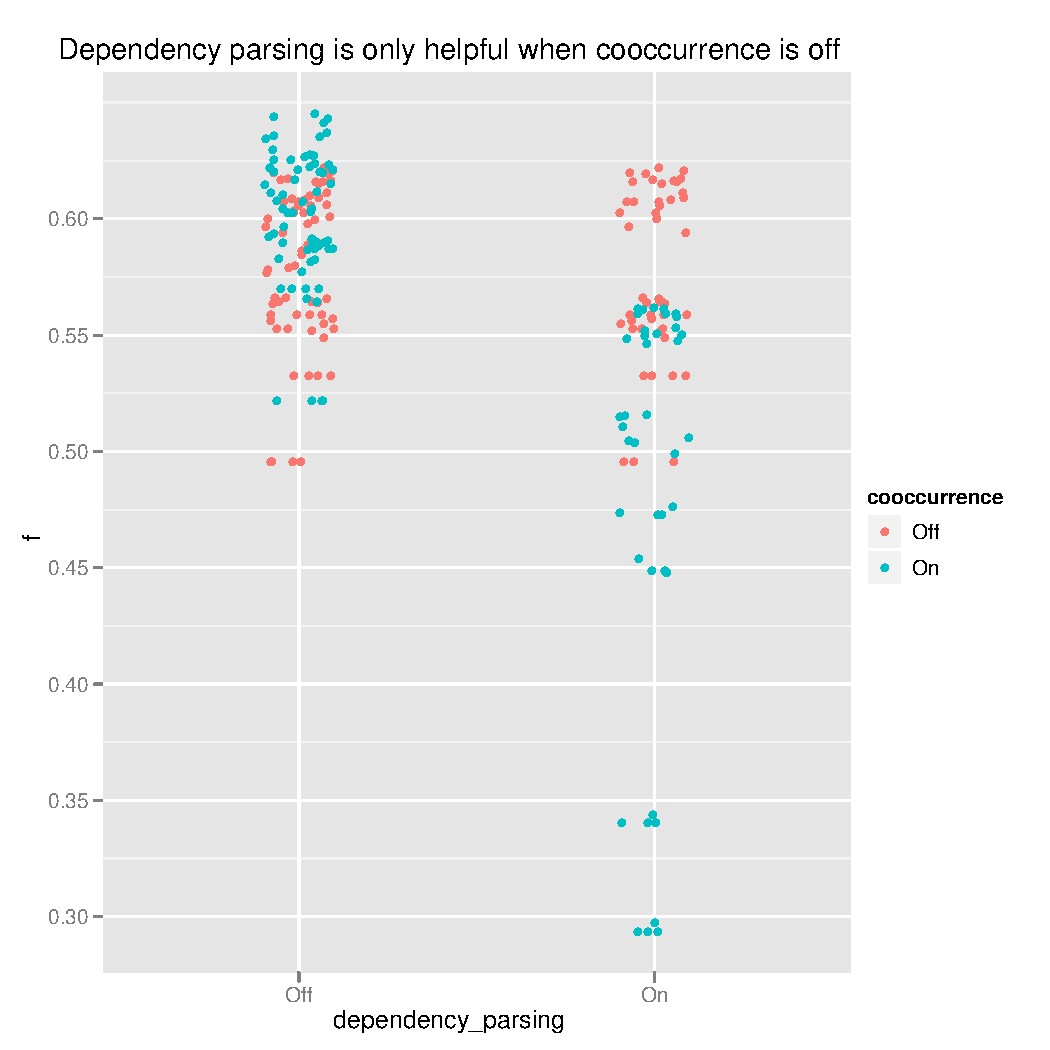
\includegraphics[width=\textwidth]{pg_0001}
\caption{\label{fig1}}
\end{figure}
>>>>>>> 148ac2b08165bf79bf456d2b556946967a1e6822

Collocation window of size 2--4 had the best performance (figure
\ref{fig2}), so we looked more closely at those. What this seems to
imply is that words very close to the head word are the most
important, as expected.

\begin{figure}[H]
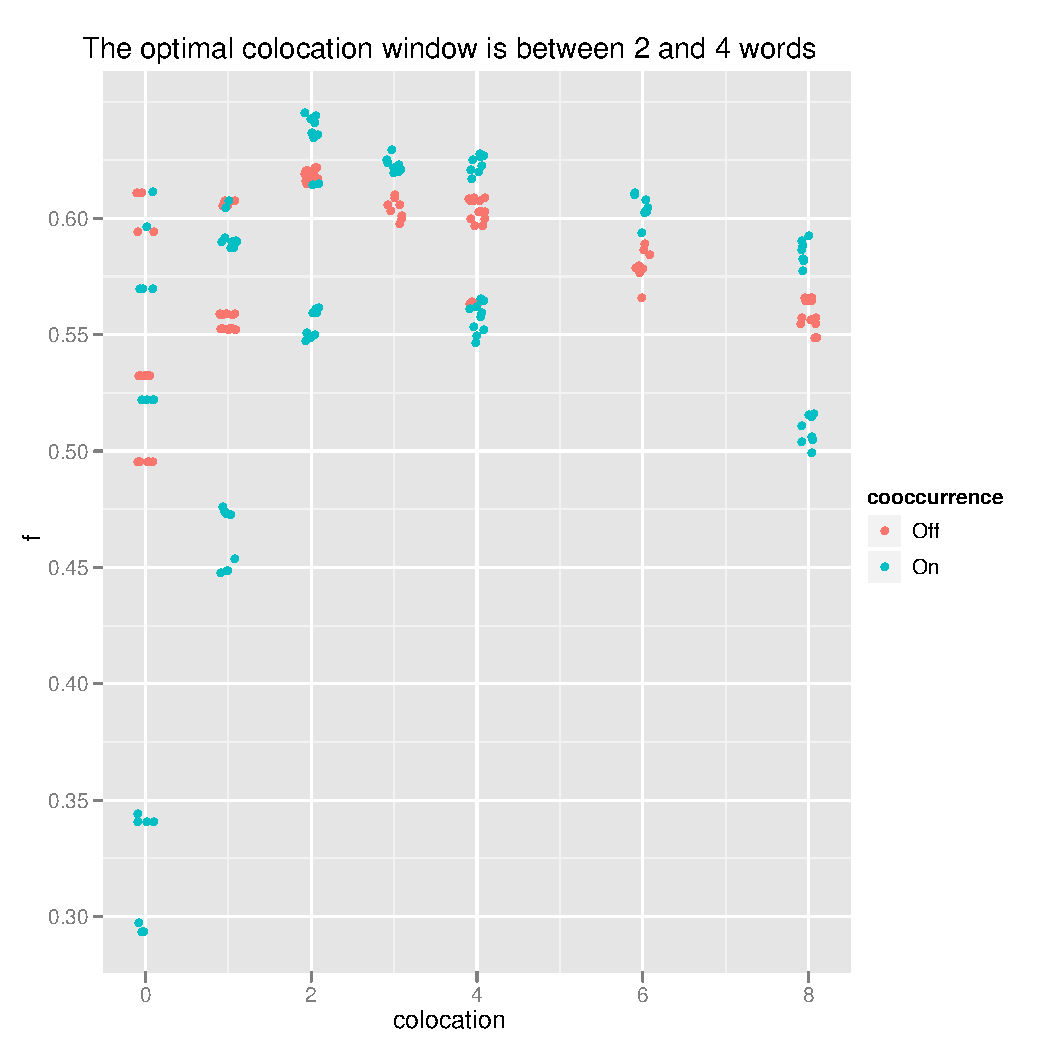
\includegraphics[width=\textwidth]{pg_0002}
%stepwise graph 1
%classifiert, collocation, cooccurrence  
%Interpret this graph
\caption{\label{fig2}}
\end{figure}

The \naive{} Bayes classifier had better top-range performance.

\begin{figure}[H]
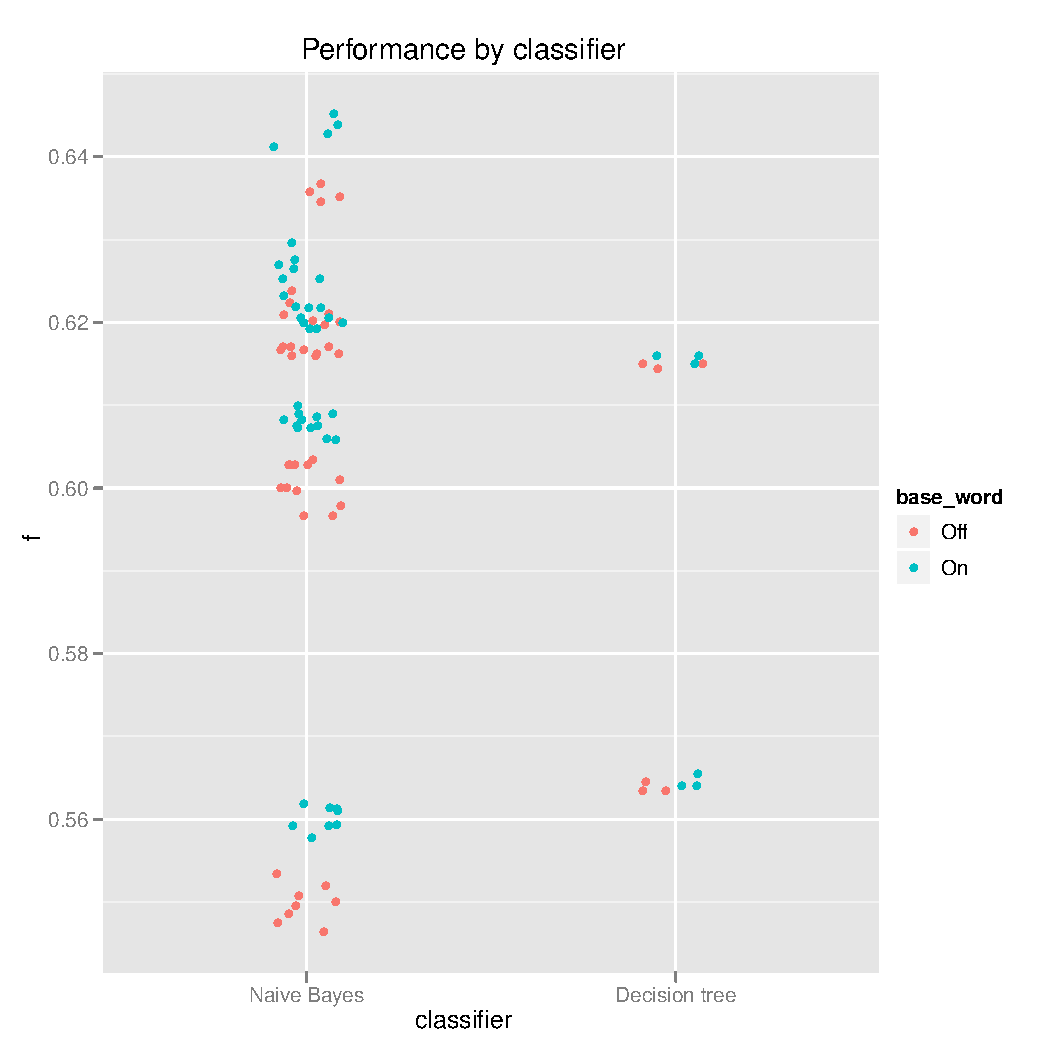
\includegraphics[width=\textwidth]{pg_0003}
\caption{\label{fig3}}
\end{figure}

\begin{figure}[H]
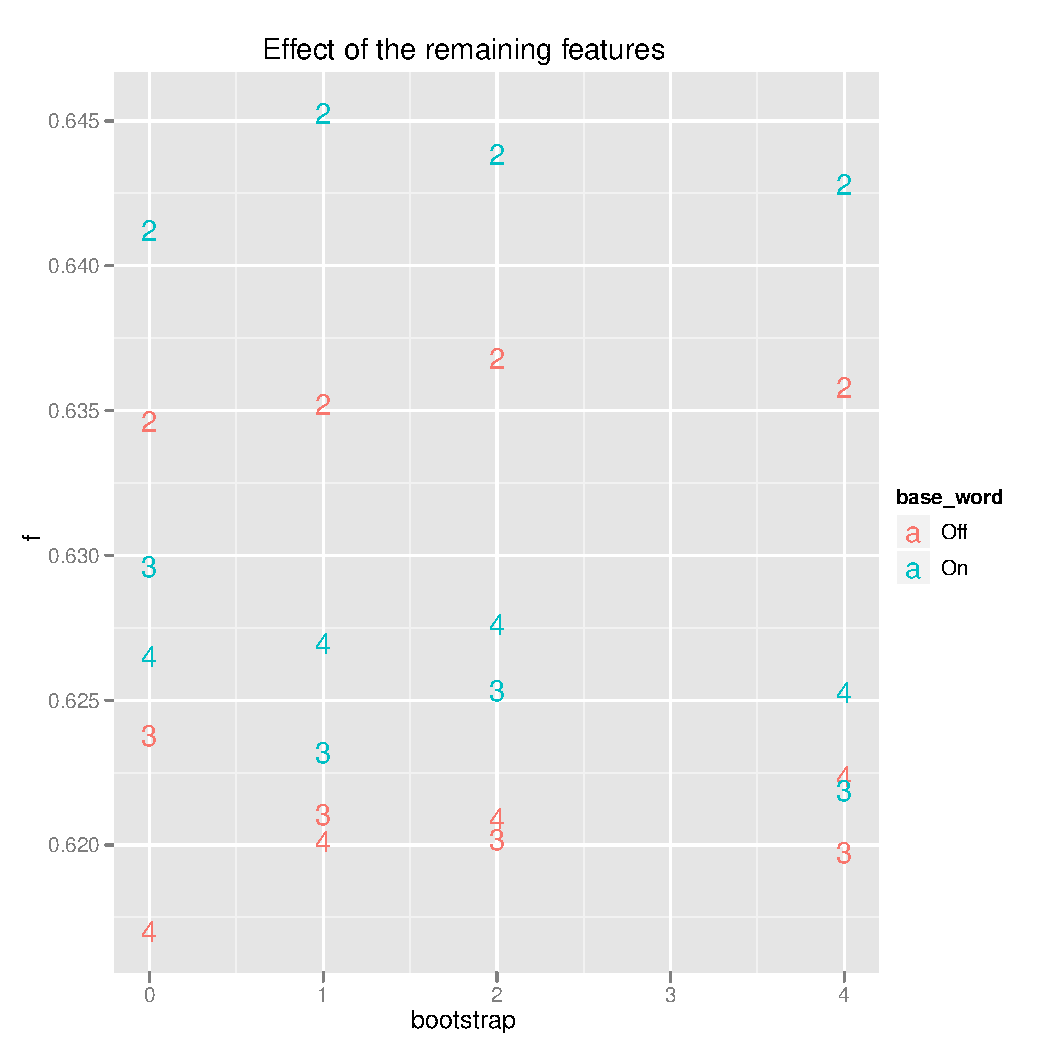
\includegraphics[width=\textwidth]{pg_0004}
\caption{\label{fig4}}
\end{figure}

\subsection{Baseline Results}

We ran two baselines, one with each machine learning algorithm:

\begin{tabular}{l l | r r r}
& grain& precision& recall& attempted\\
\hline
\multirow{3}{*}{\Naive{} Bayes} &
coarse  &  0.737 & 0.379 &   51.39\\
&mixed  &  0.730 & 0.375 &   51.39\\
& fine  &  0.693 & 0.356 &   51.39\\
\multirow{3}{*}{Decision Tree} &
coarse  &  0.612 & 0.612 &  100.00\\
&mixed  &  0.594 & 0.594 &  100.00\\
& fine  &  0.552 & 0.552 &  100.00\\
\end{tabular}

\subsection{Best Run Results}

Our run with the highest overall F-measure (overall precision 0.718, overall
recall 0.610), used co-occurrence, collocation out to a distance of 2, base word,
no dependency parsing, and bootstrapped once:

\begin{longtable}{l | r r r r r r r}
		&	&	\multicolumn{2}{c}{Fine Grain}	&	\multicolumn{2}{c}{Course Grain}	&	\multicolumn{2}{c}{Mixed}\\
Word	&	Corpus Size	&	Precision	&	Recall	&	Precision	&	Recall	&	Precision	&	Recall\\
\hline
provide.v   	&	1094	&	0.906	&	0.858	&	0.938	&	0.858	&	0.922	&	0.858\\
watch.v     	&	806 	&	0.878	&	0.851	&	0.918	&	0.851	&	0.918	&	0.851\\
remain.v    	&	1118	&	0.871	&	0.845	&	0.871	&	0.845	&	0.871	&	0.845\\
hot.a       	&	696 	&	0.853	&	0.642	&	0.853	&	0.642	&	0.853	&	0.642\\
arm.n       	&	2137	&	0.841	&	0.801	&	0.841	&	0.801	&	0.841	&	0.801\\
eat.v       	&	1463	&	0.833	&	0.816	&	0.833	&	0.816	&	0.833	&	0.816\\
add.v       	&	2148	&	0.806	&	0.777	&	0.806	&	0.777	&	0.806	&	0.777\\
plan.n      	&	1353	&	0.797	&	0.751	&	0.835	&	0.798	&	0.835	&	0.798\\
talk.v      	&	1174	&	0.797	&	0.757	&	0.797	&	0.757	&	0.797	&	0.757\\
use.v       	&	214 	&	0.786	&	0.845	&	0.786	&	0.845	&	0.786	&	0.845\\
smell.v     	&	874 	&	0.784	&	0.717   &	0.804	&	0.717   &	0.804	&	0.717\\
audience.n    	&	1637	&	0.768	&	0.750	&	0.96	&	0.947	&	0.904	&	0.907\\
expect.v    	&	1275	&	0.756	&	0.759	&	0.756	&	0.759	&	0.756	&	0.759\\
mean.v      	&	646 	&	0.737	&	0.690	&	0.737	&	0.690	&	0.737	&	0.690\\
appear.v    	&	2139	&	0.731	&	0.712	&	0.731	&	0.712	&	0.731	&	0.712\\
express.v    	&	887 	&	0.731	&	0.717   &	0.769	&	0.717   &	0.769	&	0.717\\
interest.n    	&	1489	&	0.728	&	0.636	&	0.728	&	0.636	&	0.728	&	0.636\\
sort.n      	&	1566	&	0.728	&	0.699	&	0.88	&	0.863	&	0.853	&	0.822\\
begin.v     	&	1478	&	0.723	&	0.599	&	0.723	&	0.599	&	0.723	&	0.599\\
note.v      	&	1064	&	0.712	&	0.707	&	0.712	&	0.707	&	0.712	&	0.707\\
receive.v    	&	422 	&	0.708	&	0.584	&	0.708	&	0.584	&	0.708	&	0.584\\
decide.v    	&	982 	&	0.705	&	0.700	&	0.705	&	0.700	&	0.705	&	0.700\\
wash.v      	&	534 	&	0.700	&	0.580	&	0.867	&	0.812	&	0.717	&	0.580\\
climb.v     	&	1073	&	0.698	&	0.648	&	0.698	&	0.648	&	0.698	&	0.648\\
degree.n    	&	2085	&	0.695	&	0.647	&	0.78	&	0.709	&	0.775	&	0.709\\
bank.n      	&	2113	&	0.684	&	0.598   &	0.744	&	0.658	&	0.718	&	0.628\\
ask.v       	&	2150	&	0.659	&	0.452	&	0.659	&	0.452	&	0.659	&	0.452\\
rule.v      	&	478 	&	0.655	&	0.658	&	0.655	&	0.658	&	0.655	&	0.658\\
activate.v    	&	1874	&	0.65	&	0.588	&	0.65	&	0.588	&	0.65	&	0.588\\
organization.n	&	905 	&	0.648	&	0.634	&	0.778	&	0.775	&	0.75	&	0.704\\
operate.v    	&	286 	&	0.643	&	0.438	&	0.714	&	0.658	&	0.714	&	0.658\\
hear.v      	&	510 	&	0.633	&	0.616	&	0.700	&	0.616	&	0.700	&	0.616\\
win.v       	&	631 	&	0.633	&	0.506	&	0.633	&	0.506	&	0.633	&	0.506\\
shelter.n    	&	1604	&	0.63	&	0.523	&	0.63	&	0.523	&	0.63	&	0.523\\
party.n     	&	1863	&	0.622	&	0.476	&	0.622	&	0.476	&	0.622	&	0.476\\
source.n    	&	527 	&	0.607	&	0.493	&	0.607	&	0.493	&	0.607	&	0.493\\
difference.n	&	1841	&	0.604	&	0.484	&	0.637	&	0.519	&	0.632	&	0.519\\
write.v     	&	355 	&	0.579	&	0.493	&	0.579	&	0.493	&	0.579	&	0.493\\
argument.n    	&	1831	&	0.577	&	0.355   &	0.676	&	0.426	&	0.669	&	0.426\\
atmosphere.n	&	1332	&	0.574	&	0.438	&	0.574	&	0.438	&	0.574	&	0.438\\
paper.n     	&	1914	&	0.574	&	0.303	&	0.721	&	0.371	&	0.689	&	0.371\\
lose.v      	&	574 	&	0.552	&	0.438	&	0.552	&	0.438	&	0.552	&	0.438\\
produce.v    	&	1496	&	0.538	&	0.504	&	0.538	&	0.504	&	0.538	&	0.504\\
encounter.v    	&	1046	&	0.534	&	0.486	&	0.966	&	0.850	&	0.615	&	0.546\\
image.n     	&	1176	&	0.508	&	0.426	&	0.508	&	0.426	&	0.508	&	0.426\\
disc.n      	&	1633	&	0.488	&	0.197	&	0.488	&	0.197	&	0.488	&	0.197\\
difficulty.n	&	378 	&	0.474	&	0.343	&	0.842	&	0.686	&	0.719	&	0.515\\
suspend.v    	&	1032	&	0.456	&	0.431	&	0.456	&	0.431	&	0.456	&	0.431\\
treat.v        	&	903 	&	0.442	&	0.346	&	0.465	&	0.346	&	0.465	&	0.346\\
important.a    	&	305 	&	0.438	&	0.415	&	0.562	&	0.415	&	0.531	&	0.415\\
miss.v        	&	470 	&	0.435	&	0.395	&	0.435	&	0.395	&	0.435	&	0.395\\
judgment.n    	&	502 	&	0.429	&	0.370	&	0.429	&	0.370	&	0.429	&	0.370\\
performance.n	&	1398	&	0.396	&	0.227	&	0.562	&	0.317	&	0.521	&	0.272\\
play.v        	&	838 	&	0.389	&	0.303	&	0.389	&	0.303	&	0.389	&	0.303\\
different.a    	&	796 	&	0.378	&	0.316	&	0.556	&	0.473	&	0.489	&	0.473\\
solid.a        	&	475 	&	0.25	&	0.136	&	0.25	&	0.136	&	0.25	&	0.136\\
simple.a    	&	298 	&	0.182	&	0.219	&	0.545	&	0.438	&	0.409	&	0.219\\

\end{longtable}

\section{Discussion}

\subsection{Bootstrapping}

Bootstrapping did not seem to be an effective method for improving accuracy.  This is probably because the input data is not very clean, and additionally our system is probably not very accurately estimating confidence.  When the system is not confident, it bootstraps very few examples, so it does not significantly change the model.

\subsection{Methods We Discarded}

We attempted some preliminary testing on a variety of features, but did not include them because they did not seem to provide insight:

\subsubsection{Sentence Length} For the sentence containing the word of
interest, we extracted sentence length in both characters and words. We ran two
preliminary tests to see whether this feature might be useful.

First, we used nearest-neighbor clustering to sort the lengths for a particular
word into as many groups as the word had senses. The clusters did not seem to be
related to a particular word sense; the chance of a particular instance being in
a particular group seemed to be independent of its sense.

Second, we plotted histograms sentence length. The distributions appeared to be
unimodal, further suggesting that the lengths could not be nicely grouped into
sense clusters, or any clusters for that matter.

\subsubsection{Common Words in Context}

An idea for a feature extractor was to take the most common words in a context
of a lexeme and use those words as features. Based off of the co-occurrence code,
this would generate a vector from the training data, find the most common words
from the test data, and then run the collected data through the classifier.

Unfortunately, this feature extractor did not give very good results. Both the
precision and recall for this feature extractor alone on the EnglishLS test data
were 0.039. This is to be expected since it is essentially the co-occurrence
feature extractor but without grouping data into buckets. The sparsity problem
is even more noticeable in this extractor.

\subsubsection{Part of Speech Tagging For Target Words}

We built a part-of-speech tagger and trained it on the Brown corpus. We planned
on using it to tag words, but the target words were already grouped by part of
speech, (activate.\textbf{v}) so we did not use it.


%We're using this now, just on a different corpus, right?
%\subsubsection{Bootstrapping on the Brown Corpus} 

\subsubsection{Looking through Different Corpora}

In order to get more data to use with the bootstrapping algorithm, we attempted
to search through the Brown corpus and return all of the words that were being
disambiguated in the Senseval 3 task.  To do this we needed to find all of the
instances of the words that we needed to disambiguate and return a context
(list of words) and the position of the word in that list.  We also made sure
that the context that we returned both started at the beginning of the
sentence and ended at the end of a sentence and had a minimum of 25 words
returned on either side of the word.  This data would then be converted into
the form of the data that we received from the Senseval document and ran
through the bootstrapping algorithm to have more data to train with.  However
when we actually tested this feature alone we found it to be very
uninformative.  First, there were very few instances of the words that we were
looking for (ex: activate only appeared 3 times), which made searching through
the entire corpus to find these words more time consuming than it was helpful.
Therefore, we decided not to use it for the actual test because it was not
informative enough by itself.

%The instances of the target words in the Brown corpus were very few, e.g., activate appeared only 3 times, and bootstrapping didn't seem to be very accurate in general.

\subsubsection{Dependency Parsing}

For all of its sophistication, the dependency parser didn't seem to improve
results.  This is probably because most of the relationships caught by the
parser would have been caught by the collocation feature extractor as well,
since most dependency relations are among nearby words.

\subsubsection{Collocation}

Collocation seemed to be fairly powerful at disambiguating, which is to be
expected, since function words near to the target word can be very strong
predictors of how the word is being used in context.  Effectiveness was
strongest with words close to the target, and weaker the farther away we
extended the feature.

\subsubsection{Interactions Between Features}

In principle, adding more features should not decrease our accuracy assuming
that they're at worst non-predictive, and not somehow anti-predictive, where
they fool the machine learning algorithm during training and fail spectacularly
on the test corpora.  However, because the size of the datasets is so small, it
is probable that the machine learning algorithm has too many features and too
few examples to reliably disambiguate between them, which is why we see
decreased effectiveness as we turn up the number of features, particularly with
the size of the collocation features.  This suggests that, if the training
corpus is small, it is appropriate to study which features are the most useful,
and only include those, rather than our initial approach of throwing them all
together and letting the learning algorithm sort it out.


\section{Conclusion}

The \naive{} Bayes and decision tree classifiers are not smart enough to sort out
a large number of features when the data sets are of small or moderate size,
which requires judicious choosing of features.  Co-occurrence, base word and
collocation with part of speech collocation seem to be more powerful features
than dependency parsing, and bootstrapping on the data in an attempt to get a
larger training base was ineffective because precision was too low.

\end{document}
